% \textcite
\documentclass{article}
\usepackage{amsmath,amssymb}
\usepackage{xcolor}
\usepackage{graphicx}
\usepackage{parskip}
\usepackage{xcolor}
\everymath{\color{violet}}
\usepackage[english]{babel}
\usepackage[autostyle]{csquotes}

% *** ALIGNMENT PACKAGES ***
\usepackage[margin=1.2in]{geometry}
\usepackage{times} % Font type
% *** SILENCE WARNINGS ***
\usepackage{silence}
\WarningsOff[catoptions]

% Fontsize
% \fontsize{13.5pt}{2cm}\selectfont  
\usepackage[T1]{fontenc}
\usepackage{lmodern}
\usepackage{layout}
\usepackage{titling}
\setlength{\droptitle}{-7.5em}     % Eliminate the default vertical space
\addtolength{\droptitle}{5pt}   % Only a guess. Use this for adjustment
% Definitions of handy macros can go here
\setlength{\parindent}{0pt}
\usepackage{lmodern}
\usepackage{anyfontsize} 

\usepackage[utf8]{inputenc}

\usepackage[%
  backend = biber,
  style=apa,
  citestyle=authoryear-icomp,    
  sorting=nyt,
  autocite=plain, 
  citereset=none,
  url=true,                   %URL drucken, wenn angegeben
  doi=false,                  %DOI drucken, wenn angegeben
  hyperref=true,              %Zitationen in klickbare Links
  backref=false,              %zeige in der Bibl Rücklinks 
  isbn=false,
  maxbibnames=3,  
  minbibnames=1,  
  maxnames=3,
  maxcitenames=1,
  useeditor=true,
  uniquelist=false,
  eprint=false,
  dashed=false,
  ibidtracker=false
]{biblatex}
\setlength{\bibhang}{0pt}

% % for colored citations
% \makeatletter
% \renewbibmacro*{cite:plabelyear+extradate}{%
%   \iffieldundef{labelyear}{}
%     {\clearfield{labelmonth}% don't want months in citations
%      \clearfield{labelday}% don't want days in citations
%      \clearfield{labelendmonth}% don't want months in citations
%      \clearfield{labelendday}% don't want days in citations
%      \iffieldsequal{labelyear}{labelendyear}% Don't want no-op year ranges
%        {\clearfield{labelendyear}}
%        {}%
%      \iffieldundef{origyear}
%        {}
%        {\printorigdate%
%         \setunit*{\addslash}}%
%      \iffieldundef{related}
%        {}
%        {\iffieldequalstr{relatedtype}{reprintfrom}
%          {\entrydata*{\thefield{related}}{\printlabeldateextra}%
%           \setunit*{\addslash}}
%          {}}%
%      \printlabeldateextra}}

% \renewbibmacro*{cite}{%
%   \iffieldequals{fullhash}{\cbx@lasthash}
%    {\setunit{\compcitedelim}%
%     \printtext[bibhyperref]{%
%       \usebibmacro{cite:plabelyear+extradate}}}%
%    {\printtext[bibhyperref]{%
%       \ifnameundef{labelname}
%        {\usebibmacro{cite:noname}%
%          \setunit{\printdelim{nameyeardelim}}%
%          \usebibmacro{cite:plabelyear+extradate}%
%          \savefield{fullhash}{\cbx@lasthash}}
%        {\ifnameundef{shortauthor}
%          {\printnames{labelname}}%
%          {\cbx@apa@ifnamesaved
%            {\printnames{shortauthor}}
%            {\ifnameundef{groupauthor}
%              {\printnames[labelname]{author}}
%              {\printnames[labelname]{groupauthor}}%
%             \addspace\printnames[sabrackets]{shortauthor}}}%
%          \setunit{\printdelim{nameyeardelim}}%
%         \usebibmacro{cite:plabelyear+extradate}%
%         \savefield{fullhash}{\cbx@lasthash}}}}%
%    \setunit{\multicitedelim}}

% \renewbibmacro*{textcite}{%
%   \iffieldequals{fullhash}{\cbx@lasthash}
%     {\setunit{\compcitedelim}%
%      \printtext[bibhyperref]{%
%        \usebibmacro{cite:plabelyear+extradate}}}
%     {%
%     \ifbool{cbx:parens}
%       {\bibcloseparen\global\boolfalse{cbx:parens}}
%       {}%
%       \setunit{\compcitedelim}%
%       \ifnameundef{labelname}
%        {\iffieldundef{shorthand}%
%          {\printtext[bibhyperref]{%
%             \usebibmacro{cite:noname}}%
%           \setunit{\ifbool{cbx:np}%
%                    {\printdelim{nameyeardelim}}%
%                    {\global\booltrue{cbx:parens}\addspace\bibopenparen}}%
%           \printtext[bibhyperref]{%
%             \usebibmacro{cite:plabelyear+extradate}}}
%          {\printtext[bibhyperref]{%
%             \usebibmacro{cite:shorthand}}}}
%        {\printtext[bibhyperref]{%
%           \ifnameundef{shortauthor}%
%            {\printnames{labelname}}
%            {\cbx@apa@ifnamesaved
%              {\printnames{shortauthor}}
%              {\ifnameundef{groupauthor}
%                {\printnames[labelname]{author}}
%                {\printnames[labelname]{groupauthor}}}}}%
%         \setunit{\ifbool{cbx:np}
%                   {\printdelim{nameyeardelim}}
%                   {\global\booltrue{cbx:parens}\addspace\bibopenparen}}%
%         \printtext[bibhyperref]{%
%           \ifnameundef{shortauthor}
%            {}
%            {\cbx@apa@ifnamesaved
%              {}
%              {\printnames{shortauthor}\setunit{\printdelim{nameyeardelim}}}}%
%           \usebibmacro{cite:plabelyear+extradate}}%
%         \savefield{fullhash}{\cbx@lasthash}}}}
% \makeatother

\addbibresource{citations.bib} %Imports bibliography file

\definecolor{reddish}{HTML}{B6301C}
\definecolor{blueish}{HTML}{001473}
\usepackage[colorlinks=true, citecolor=blueish, linkcolor=reddish]{hyperref}

\DeclareMathOperator*{\argmax}{argmax} % thin space, limits underneath in displays

\title{The Bayes' Theorem}

\author{Rel Guzman}
\date{February 2023}


\begin{document}

\maketitle

From statistics to finance to cutting-edge robotic systems, a theorem that comes up frequently is the \textit{Bayes' theorem}, which was originally developed by Thomas Bayes—a British statistician and Presbyterian minister—back in the 18th century \parencite{andersson2022introduction}. The Bayes' theorem is denoted as follows:
\begin{align}
\operatorname{Posterior} = \frac{\operatorname{Likelihood} \cdot \operatorname{Prior}}{\operatorname{Evidence}}~.
\end{align}

Thomas Bayes was a British statistician and mathematician who is best known for his work in probability theory. In general, \textit{probability theory} provides mathematical tools for dealing with \enquote{degrees of belief} \parencite{russell2010artificial} about events such as the probability of having a cold. Probability theory is used for modeling reasoning and decision-making under uncertainty according to what is known as a probability model, which leads to a predictive model when the purpose of the model is to make predictions about certain events. For example, a simplistic medical diagnosis problem may consist of determining the cause of a headache. A predictive model can determine the cause of a headache by defining a set of possible causes $\operatorname{Headache} \Rightarrow \operatorname{Cold} \lor \operatorname{BadPosture} \lor \operatorname{Alcohol}$; however, we cannot be completely sure of what a patient has! We can only provide a degree of belief about each cause by defining random variables: a symptom variable $X$ with possible values $\{x_1=\operatorname{Headache}, x_2=\operatorname{NotHeadache}\}$ and a cause variable $Y$ with possible values $\{y_1=\operatorname{Cold}, y_2=\operatorname{BadPosture}, y_3=\operatorname{Alcohol}\}$. Probability theory allows us to define a \textit{posterior probability} for having a cold given that we have a headache denoted as $p(\operatorname{Cold} \mid \operatorname{Headache})$. Such a probability can be found by applying the Bayes' theorem
\begin{align}
p(Y=\operatorname{Cold} \mid X=\operatorname{Headache}) = \frac{p(X=\operatorname{Headache} \mid Y=\operatorname{Cold}) p(Y=\operatorname{Cold})}{p(X=\operatorname{Headache})}~.
\end{align}

 % p(Y\mid X) = \frac{p(X\mid Y)p(Y)}{p(X)}


Assuming a data set is collected from several patients: Patients with a cold that got a headache $p(\operatorname{Headache} \mid \operatorname{Cold})$, and patients with a cold $p(\operatorname{Cold})$, the posterior probability can be computed. To generalize, the most probable cause can also be calculated by applying the formulation:
\begin{align}
y^* = \argmax_{y} p(Y=y)\prod_{i=1}^n p(X=x_i\mid Y=y)~.
\end{align}

which is the basis for what is known as \textit{Bayesian machine learning}, which corresponds to learning predictive models using the Bayes' theorem. In turn, learning corresponds to optimizing a function $y = f(\mathbf{x})$, where $\mathbf{x} = (x_1, x_2, \ldots, x_d)$ is a $d$-dimensional input. Functions can be as complex as the function from \autoref{fig:complexfunction}. For example, minimizing the difference between a generated image and a real image, which is the principle of generative adversarial networks (GAN) \parencite{gonog2019review}.

\begin{figure}[h]
    \centering
    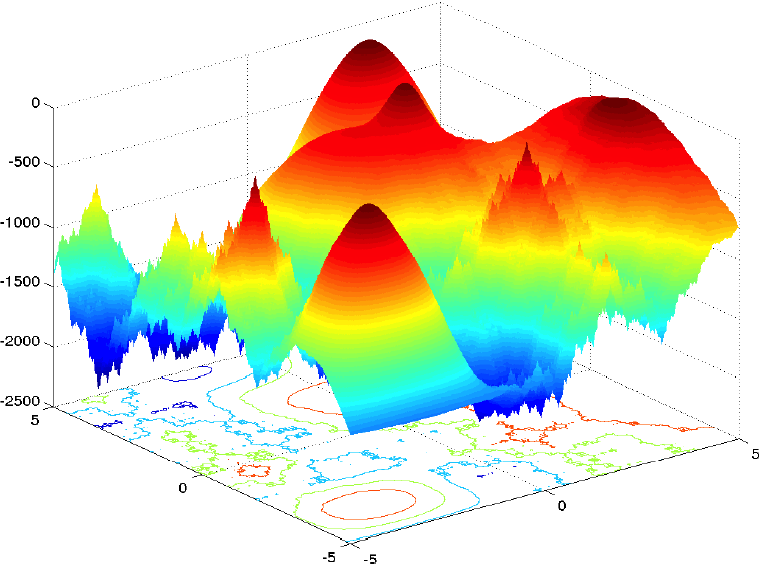
\includegraphics[width=0.6\textwidth]{figures/complexfunction.png}
    \caption{Nonlinear, two-dimensional function with multiple local optima. Source: \parencite{li2013benchmark}}
    \label{fig:complexfunction}
\end{figure}

For example, the difference between optimizing $f$ with gradient-based optimization methods suggested in \textcite{bengio2000gradient} and optimizing $f$ with a Bayesian approach is that a \textit{posterior probability distribution} can be obtained with the latter. In the diagnosis example, not only can we know the probability that the cause is a $\operatorname{Cold}$ but also the probability that the cause is $\operatorname{BadPosture}$ and so on, which allows handling uncertainty. A similar type of inference happens when optimizing complex functions. In fact, there is a method known as \textit{Bayesian optimization (BO)} \parencite{shahriari2015taking} where a function posterior $p(f \mid \mathcal{D})$ can be optimized where $\mathcal{D}$ is a collected dataset composed of pairs $(\mathbf{x}, y)$. Bayesian machine learning is also applied to powerful deep learning approaches, such as the use of \textit{Bayesian neural networks} \parencite{jospin2022hands}. 

The main advantages of Bayesian machine learning come up when measuring uncertainty is necessary and when optimizing learning models in low data availability situations. Besides measuring uncertainty as in the diagnosis example, uncertainty is also useful when optimizing complex functions where there can be a trade-off between exploring unseen regions (where uncertainty is high) and exploiting current solutions \parencite{Luke2013Metaheuristics}. One of the fields where data availability is a big issue is the field of robotics because of the costly performance functions to evaluate in the real world \parencite{shahriari2015taking}. 

To summarize, the Bayes theorem is widely used when dealing with uncertainty due to its ability to optimize functions with the use of random variables and probability theory. Its use in complex fields makes Bayesian methods undeniably useful.

% collected for computing the probabilities.

% Given collected data, for example, 

% Inferring 

% Calculating such a probability happens to be possible only by doing what 

% the learning process consists of building a probability $p(y| x)$ that describes a conditional probability distribution of $y$ given the input $x$, and such probability $p(y| x)$ can be learned either discriminatively or generatively.

% generative predictive model. 

% From a Bayesian approach, the probability distribution $p(\mathbf y| \mathbf x)$ is the quantity of interest called the \textit{posterior}, and it can be estimated through the application of the Bayes' rule, considering the variable dependency

% This is due to the applicability of such a mathematical formulation

\printbibliography


\end{document}
